\chapter{Iteración 3: Primer prototipo de Hardware} % (fold)
\label{cha:iteracion_3}


\section{Introducción} % (fold)
\label{sec:introduccion}

Una vez terminada la iteración 1 (donde definimos los componentes físicos a utilizar), y teniendo en cuenta que en el Laboratorio de Arquitectura de Computadoras (LAC) había una placa de desarrollo de SiliconLabs (modelo C8051f352DK) con gran cantidad de los componentes que nosotros necesitábamos para nuestro desarrollo. Lo que decidimos fue basar y adaptar nuestro diseño a la C8051f352DK, para minimizar los errores.

En esta iteración realizamos el diseño y construcción de una placa de desarrollo que cumpla con los requerimientos planteados.


%la primera placa que fue una verga. tenia el rs232, tenia 8 entradas, tenia la alimentacion separada de la entrada para la programacion del micro. osea podia alimentarse mediante el debugger o alimentacion externa. se adapto el diseño de la placa para poder programar el micro con el debugger de silicon labs. hay que tener en cuenta que nos basamos en el diseño hecho por silicon labs de la placa de desarrollo c8051f352 que teniamos en el lac. la vamos a haber construido en esta iteracion, y lo unico que llego a hacer fue conectarse con la ide. nada mas, el resto no anduvo nada. %

% section introduccion (end)

\section{Requerimientos de la iteracion} % (fold)
\label{sec:requerimientos_de_la_iteracion}

Diseñar y construir un prototipo de placa con las siguientes características:

\begin{itemize}
\item El circuito debe incluir en su diseño aquellos requisitos de hardware impuestos por el mismo microcontrolador(?)
\item Al circuito se le deben poder conectar 8 entradas analógicas.
\item Al circuito se le deben poder conectar 4 entradas de eventos digitales externos.
\item Las entradas analógicas deben tener filtros para mejorar la inmunidad al ruido.
\item Se debe incluir en el diseño el circuito necesario para soportar comunicación vía RS232
\item La placa debería poder alimentarse a través de una fuente de tensión externa.
\item Se debería poder conectar el debugger del microcontrolador a la placa para poder programarlo.
\item El circuito de programación del microcontrolador debería estar separado la placa principal.
\end{itemize}


% section requerimientos_de_la_iteracion (end)

\section{Desarrollo} % (fold)
\label{sec:desarrollo}

\subsection{Elección de Herramientas para Diseño} %(fold)
\label{sec:herramientas_para_diseno}

Gracias a que en el LAC en dicho momento estaba realizando trabajos Santiago Rodríguez (Ingeniero en Computación, egresado de la UNC), pudimos consultar con él sobre el diseño y desarrollo de placas PCB. 

Santiago nos recomendó utilizar varias herramientas para el diseño:
\begin{itemize}
\item Kicad.
\item Altium Designer.
\item Eagle.
\item PCBwizard.
\end{itemize}

Ademas para poder realizar la impresión de la placa PCB en la fresadora que tiene el LAC, ProtoMat E33 de LPKF, necesitamos tener instalado el software de la empresa, llamado LPKF Circuit Pro PM.

Luego de probar las herramientas para diseñar la placa, nos terminamos decidiendo por Kicad, ya que fue el mas sencillo de utilizar, mas amigable su interfaz y era el que nos exportaba los archivos que necesitábamos para poder utilizar el Circuit Pro e imprimir la placa en la Fresadora.

%subsection herramientas_para_diseno (end)

\subsection{Diagramas de Bloques de Hardware}
\label{diagra_bloques_hardware}

La primera etapa de diseño consiste en realizar un diagrama de bloques que, en base a los requerimientos planteados para esta iteración, ilustre a grandes rasgos la organización del circuito que pretendemos realizar.
Podemos ver en la figura \ref{fig:BloquesHardw1} el diagrama de bloque que hicimos.

\begin{figure}[h]
  \centering
  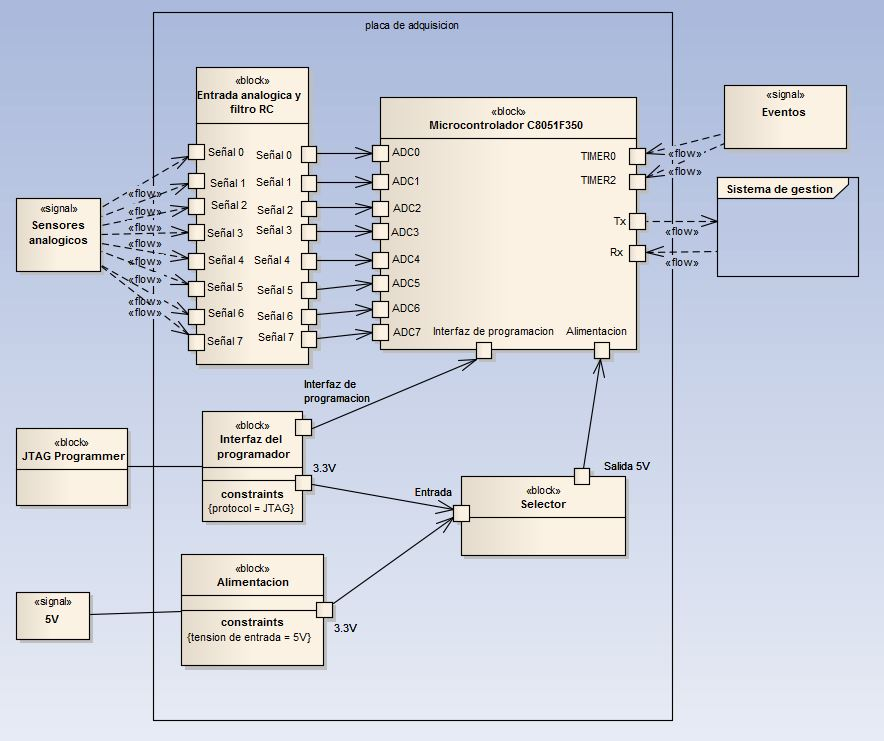
\includegraphics[width=0.50\textwidth, height = 7cm]{BloquesHardw1}
  \caption{Diagrama de Bloque de la Placa.}\label{fig:BloquesHardw1}
\end{figure}

Los bloques en la figura 5 representan de forma general los distintos módulos a implementar. Las entradas analógicas se introducen al sistema (microcontrolador) a través de filtros reductores del ruido (filtros RC). Luego, las señales, son procesadas por el microcontrolador (C8051f352). El bloque de GPIO y contadores de eventos es simplemente un grupo de pines direccionados a distintas entradas del microcontrolador, GPIO significa "General Purpose Input Output"(en español, "entrada y salida de propósito general" ). Son 4 pines que se separaron para uso general, por necesidad eventual de necesitarlos. Parte de estos GPIO son los pines contadores de eventos, por lo cual se incluyeron dentro del mismo bloque.

Es posible alimentar el sistema por medio del programador o debugger (propietario de Silicon Labs), o mediante una fuente de tensión externa de 5V, que al pasar por un regulador de tensión disminuye su voltaje a 3.3V para llegar al nivel de tensión del C8051f352. Ademas tendrá una llave selectora donde decidimos si se alimenta el sistema usando la fuente continua de 5V, o utilizando el programador.

%subsection diagra_bloques_hardware (end)

\subsection{Diseño Esquemático}
\label{diseno_esquematico}

Para poder realizar el diseño esquemático del circuito utilizamos el software KiCad. Para simplificar la explicación del diagrama, lo que haremos en esta sección es dividir el circuito entero en subcircuitos mas simples. Al final mostraremos el sistema final.

\subsubsection{Entradas Analógicas}
\label{entradas_analogicas}

El circuito contiene 8 entradas analógicas iguales cada una, por lo que mostraremos el ejemplo de una sola entrada. Podemos ver en la figura  el circuito para la entrada de la señal. 

Sabemos que la señal entra al sistema con ruido (ya sea como interferencia de señales externas, o ruido provocado por los mismos componentes del circuito). Por lo que como primera medida, se aplica a la señal de entrada un filtro RC pasivo, pasa bajo. Así introducimos muy poca atenuación a las frecuencias que son menores que la frecuencia de corte. Las frecuencias que son mayores que la de corte son atenuadas fuertemente. 
Como podemos ver en la figura \ref{fig:Entrada_y_filtro} tenemos un pin (AI0) de entrada para conectar la salida de un sensor analógico, seguido de un filtro RC, compuesto por una resistencia de 100 ohms, y un capacitor a tierra de 0,1 microFaradios. La salida de la resistencia esta conectada directamente a la entrada AIN0.0 del C8051f352.

\begin{figure}[h]
  \centering
  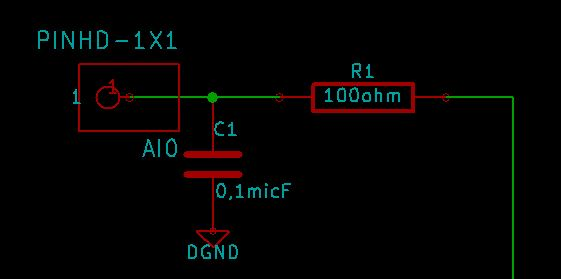
\includegraphics[width=0.70\textwidth, height = 4cm]{Entrada_y_filtro}
  \caption{Esquemático del circuito de entrada analógica, más filtro RC pasa-bajo.}\label{fig:Entrada_y_filtro}
\end{figure}

%subsubsection entradas_analogicas (end)

\subsubsection{Circuito Salida Serial}
\label{salida_serial}

Uno de los requerimientos de esta iteración es que la placa a desarrollar debe soportar comunicación serial, así que propusimos que dicha comunicación sea vía RS-232.

Como el nivel de tensión que entrega la salida serial TTL del microcontrolador C8051f352 es distinta a la necesaria para aplicar el protocolo RS-232. Nos vimos obligados a realizar un circuito para adaptarlo, y así asegurar el correcto envío de datos. Para realizar dicho circuito se utilizó el integrado MAX232 y se configuró como se muestra en la figura \ref{fig:MAX232}. Como podemos ver se utilizaron Capacitores de 0,1 microFaradios. Los pines "XRX1", "XCTS1", "XTX1" y "XRTS1" son los que tendrá el modulo de salida RS-232.
Ademas colocamos 4 jumpers (JP1, JP2, JP3, JP4) a la entrada del MAX232 por si se necesita la salida TTL del microcontrolador (por ejemplo si se quiere conectar la salida serial a un arduino o raspberry pi).

La tensión para alimentar el integrado es de 3.3V que se sacan del sub-circuito de potencia que se explicara en \ref{sub}.

\begin{figure}[h]
  \centering
  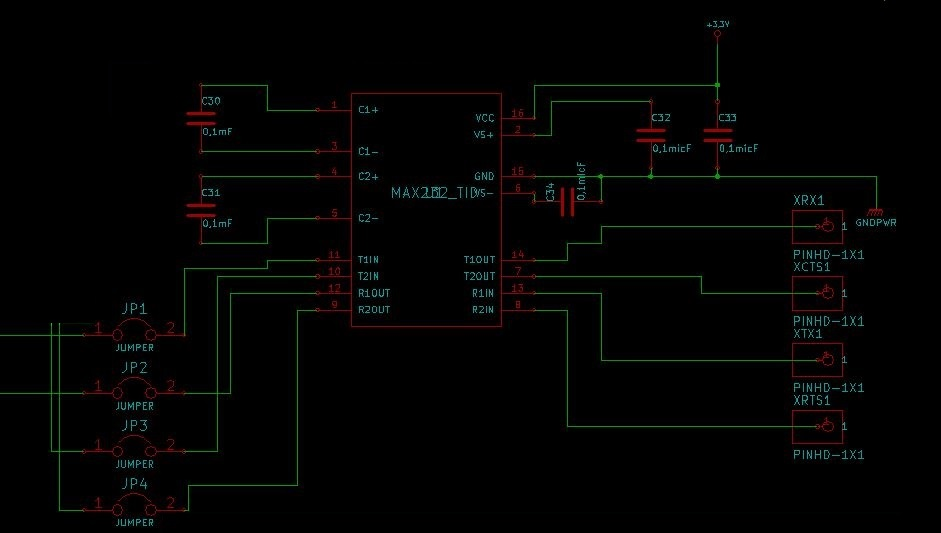
\includegraphics[width=0.80\textwidth, height = 11cm]{MAX232}
  \caption{Esquemático del Circuito MAX232 .}\label{fig:MAX232}
\end{figure}

%subsubsection salida_serial (end)

\subsubsection{Circuito de Potencia}
\label{circuito_potencia}

Del análisis del microcontrolador y de otros componentes que necesitamos utilizar en la placa(como MAX232, leds, etc), decidimos realizar separar el circuito de potencia para dividir la tensión en dos de distintos valores: 3,3V y 5V.
Como podemos ver en la figura \ref{} el sistema de alimentación lo implementamos a través de un Jack de Power (Jack2P) para conectar una fuente de tensión de 5V, y a través del programador/debugger de Silicon Labs 5V(Debugger1). A continuación colocamos un jumper de 3 pines para poder seleccionar el método de alimentación (Jumper1).

\begin{figure}

\end{figure}

Para poder alimentar al microcontrolador necesitábamos 3.3V así que utilizamos un regulador de tensión (LM2937). El C8051f352 tiene dos entradas de alimentación, una analógica y una digital, ambas con un rango entre 2.9V a 3.6V, ademas la corriente puede variar entre 5.7mA (en estado inactivo) hasta 11.3mA (en estado activo). Es por ello que se colocan las resistencias, y ademas se colocan capacitores en paralelo para disminuir el ruido de entrada.

%subsubsection circuito_potencia (end)

\subsubsection{Diagrama Esquematico Final}
\label{esquematico_final_1}

En la figura \ref{fig:EsquematicoCompleto1} se puede ver el diagrama de la placa completo. 
Podemos distinguir un apartado donde hay dos ferrite brides para dividir la masa analógica de la masa digital y así evitar ruidos para la conversión del ADC, debido a posibles frecuencias altas.

\begin{figure}
\centering
  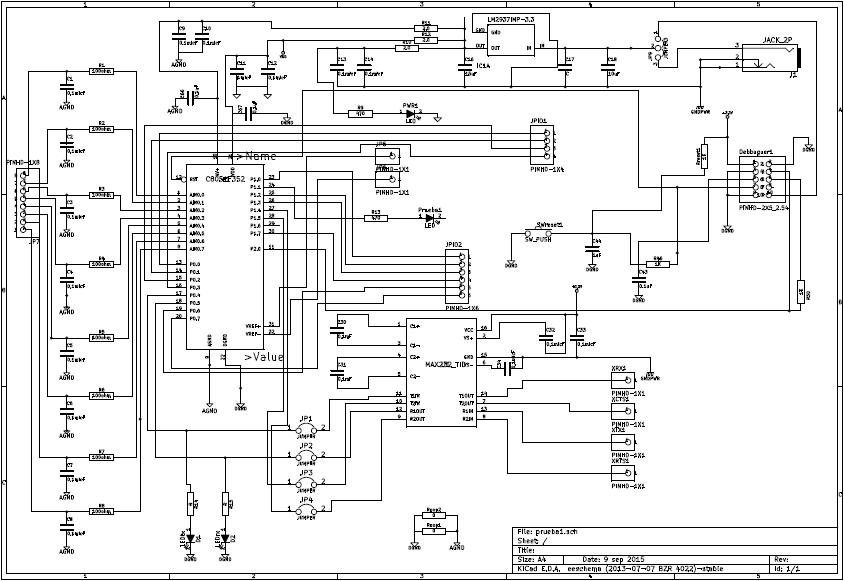
\includegraphics[width=1.10\textwidth, height = 12cm]{EsquematicoCompleto1}
  \caption{Esquemático del Circuito Completo de la placa.}\label{fig:EsquematicoCompleto1}
\end{figure}

%subsubsection esquematico_final_1 (end)

%subsection diseno_esquematico (end)

\subsection{Diseño de Plaqueta de Circuito Impreso (PCB)}
\label{pcb1}

En electrónica, plaqueta de circuito impreso (printed circuit board, PCB), es la superficie constituida por caminos o pistas de material conductor laminadas sobre una base no conductora. El circuito que se imprime en un plaqueta se utiliza para interconectar distintos dispositivos electrónicos.

En el Laboratorio de Arquitectura de Computadoras hay instalada una fresadora para la impresión de placas PCB, el modelo es LPKF E33, por lo que el software que utilizamos fue "Circuit Pro" que es propietario de LPKF, así nos aseguramos la compatibilidad de archivos y drivers.

En la figura \ref{fig:} podemos ver como quedo el diseño del circuito PCB:

\begin{figure}

\end{figure}


%subsection pcb1 (end)

% section desarrollo (end)

\section{Pruebas} % (fold)
\label{sec:pruebas}

%Prueba 1: Con el diseño PCB hecho, chequear los errores ERC(perfom design rules check)de KiCad para fijarse si todos los componentes estén interconectados como tiene que estar.
%Resultado1: Se eliminaron todos los errores ERC 
%Prueba 2: Con la placa ya impresa, testeo de todas las pistas ruteadas, con un multimetro seteado para medir continuidad, así chequeamos si existen cortocircuitos por fallos de la fresadora.
%Resultado 2: No se encontraron cortos por fallo de la fresadora.
%Prueba 3: Con la placa ya impresa,y los componentes soldados, testeo de todas las pistas ruteadas, con un multimetro seteado para medir continuidad, así chequeamos cortocircuitos por fallos de soldaduras.
%Resultado 3: Se encontraron cortocircuitos causado por malas soldaduras, que gracias a la malla desoldadora los pudimos solucionar, se realizo la prueba 3 de nuevo y no se encontraron mas cortocircuitos. 
%Prueba 4: Con la placa ya impresa,y los componentes soldados, conectamos el debugger de SiliconLabs y conectamos a PC, para chequear si la IDE se puede comunicar con el microcontrolador.
%Resultado 4: Cuando conectamos la placa a la PC, la IDE de SiliconLabs pudo reconocer el microcontrolador.
%Prueba 5: Con la placa ya impresa,y los componentes soldados, y la IDE reconociendo el microcontrolador, intentamos cargar un programa (.hex) al C8051f352.
%Resultado 5: Conectamos la placa a la PC, pero al momento de cargar el programa, la IDE tira un error con la flash del microcontrolador. No pudimos resolver este problema en esta iteración.

\begin{table}[h]
\caption{Test de sistema 1}
\label{tab:testsistema1}
\begin{tabular}{p{2cm} p{9cm}}
\multicolumn{2}{c}{\cellcolor[HTML]{68CBD0}{\color[HTML]{000000} Prueba de sistema}}                                                                                                                                                                                                                                                   \\
Prueba \#        & 1                                                                                                                                                                                                                                                                                                                   \\
\hline
Nombre           & Correcto Diseño de PCB.                                                                                                                                                                                                                                                           \\
\hline
Descripcion      & Se chequea si existen errores en el diseño utilizando el ERC (perfom design rules check) que provee el KiCad.                                                                                   \\
\hline
Pre-condiciones  & \tabitem Componentes colocados y ruteados. \\
                 & \tabitem Pads numerados con sus etiquetas.  \\
\hline

Post-condiciones & El resultado de ERC debe ser cero.                     
\\
\hline
Resultados       & No se encuentrar errores de diseño en el PCB.                                                                                       
\end{tabular}
\end{table}

\begin{table}[h]
\caption{Test de sistema 2}
\label{tab:testsistema2}
\begin{tabular}{p{2cm} p{9cm}}
\multicolumn{2}{c}{\cellcolor[HTML]{68CBD0}{\color[HTML]{000000} Prueba de sistema}}                                                                                                                                                                                                                                                   \\
Prueba \#        & 2                                                                                                                                                                                                                                                                                                                   \\
\hline
Nombre           & Correcta impresion de la placa.                                                                                                                                                                                                                                                          \\
\hline
Descripcion      & Corroboramos que todas las pistas y que todos los drills se hayan impreso. Luego con un multimetro seteado en cuntinuidad comprobamos que no existan cortocircuitos entre pistas y masa o entre pads y masa.                                                                                  \\
\hline
Pre-condiciones  & \tabitem Placa impresa. \\
                 & \tabitem Multimetro seteado en continuidad.\\
\hline

Post-condiciones & La placa debe tener las mismas pistas que aparecen en el diseño de PCB, y al medir con el tester nunca debe dar continuidad entre masa y pistas, o entre pads y pistas.  
\\ 
\hline
Resultados       & Todas las pistas estaban de acuerdo con el PCB. Al medir la continuidad de las pistas se encontraron algunos cortuciruitos producidos por una mala colocacion del la plancha al momento de la impresion. Se solucionaron volviendo a imprimir la placa.                                                                                                                                                   
\end{tabular}
\end{table}

\begin{table}[h]
\centering
\caption{Test de sistema 3}
\label{tab:testsistema3}
\begin{tabular}{p{2cm} p{9cm}}
\multicolumn{2}{c}{\cellcolor[HTML]{68CBD0}{\color[HTML]{000000} Prueba de sistema}}                                                                                                                                                                                                                                                   \\
Prueba \#        & 3                                                                                                                                                                                                                                                                                                                   \\
\hline
Nombre           & Correcta soldadura de Componentes                                                                                                                                                                                                                                                         \\
\hline
Descripcion      & Se utiliza el multimetro seteado en continuidad para poder chequear si existen cortocircuitos y para saber si todos los componentes estan bien interconectados.                                                                                  \\
\hline
Pre-condiciones  & \tabitem Placa impresa. \\
                 & \tabitem Pistas impresas correctamente. \\
                 & \tabitem Componentes soldados. \\
                 & \tabitem Multimetro seteado en continuidad. \\
\hline

Post-condiciones &  No deben encontrarse cortocircuitos, y deben comprobarse la continuidad de las interconexiones de componentes.
\\ 
\hline
Resultados       & Se encontraron cortocircuitos luego de soldar los componentes, al intentar solucionarlo las pistas se rompieron. Para solucionar este problema volvimos a imprimir la placa, realizamos la prueba de sistema 2 de vuelta y soldamos todos los componentes, realizamos esta prueba de nuevo y no encontramos ningun cortocircuito.                                                                                                                                                     
\end{tabular}
\end{table}



% section pruebas (end)

\section{Resultados} % (fold)
\label{sec:resultados}
En las siguientes imágenes podremos ver el resultado final de la placa.

\begin{figure}[H]
  \centering
  \includegraphics[width=0.80\textwidth, height = 10cm]{resultadohardware1}
  \caption{Placa completa con todo sus componentes soldados.}\label{fig:resultadohardware1}
\end{figure}

En esta iteración cumplimos con los requerimientos planteados, construyendo una placa con un C8051f352, que contenga 8 señales analógicas de entrada y 4 entradas digitales. Le pudimos colocar una salida serial para conectar a una PC.
Logramos alimentar por una fuente de tensión externa o con el debugger de SiliconLabs. El microcontrolador fue reconocido por la IDE de SiliconLabs cuando era conectado por el debugger en la PC, pero no pudimos cargarle un programa al c8051f352, ya que nos daba error con la memoria flash.
% section resultados (end)

% chapter iteracion_3 (end)